\section{Proposed VAE-accelerated EM-aware IR drop fixing method}
\label{sec:strategy}

\subsection{EM-Aware IR Drop Prediction}
\label{subsec:emvae}

\subsubsection{AEs, VAEs, and CVAEs}
\label{subsec:vae_intro}

CNNs with an encoder-decoder structure are widely used in image generation tasks. 
 This architecture forms the basis for several generative models, including the simplest form AutoEncoders (AEs), Generative Adversarial Networks (GANs), and Variational AutoEncoders (VAEs)~\cite{Diederik:arxiv'22}. 
GAN ~\cite{Goodfellow:NIPS'14} model introduces an additional binary output CNN called \textit{discriminator} only during the training stage to improve the result quality, and adopts the same AE structure for result generation.Fig.\ref{fig:ae}  shows AEs (GANs) encode input $\textbf{x}$ to low-dimensional latent variables $\textbf{z}$ by the encoder and then decode the result by the decoder.


VAE, as shown in Fig.\ref{fig:vae}, is a unique generative model derived from the standard AE. Compared to the traditional AE structure, VAE does not encode the input into a discrete point, but a distribution over the latent space $Q(Z|X)$ with multivariate Gaussian prior. This enables the VAEs to have a better latent space interpretability.
%which is used to generate new data similar to the input data it's trained on. 
%This step is crucial to the VAE's characteristics over AE and AE-based GAN models, such as latent space  interpretability, and training stability.
%which means that the latent space is smooth and interpretable, enabling ability to interpolate between different points in the latent space and generate new samples that exhibit a smooth transition between the characteristics of the original points. On the other hand, AE does not explicitly enforce such a structure, making the latent space less interpretable and interpolations might not always produce meaningful outputs. 

Building upon the foundation of VAEs,  we propose to adopt the CVAE as the backbone, which extends the VAE to incorporate the conditional information, including the given aging time and current map, so that our model can predict the EM-aware IR drop conditioned on the specified aging time and current distribution. 

\begin{figure}[htp]
	\centering
	\subfigure[]{
		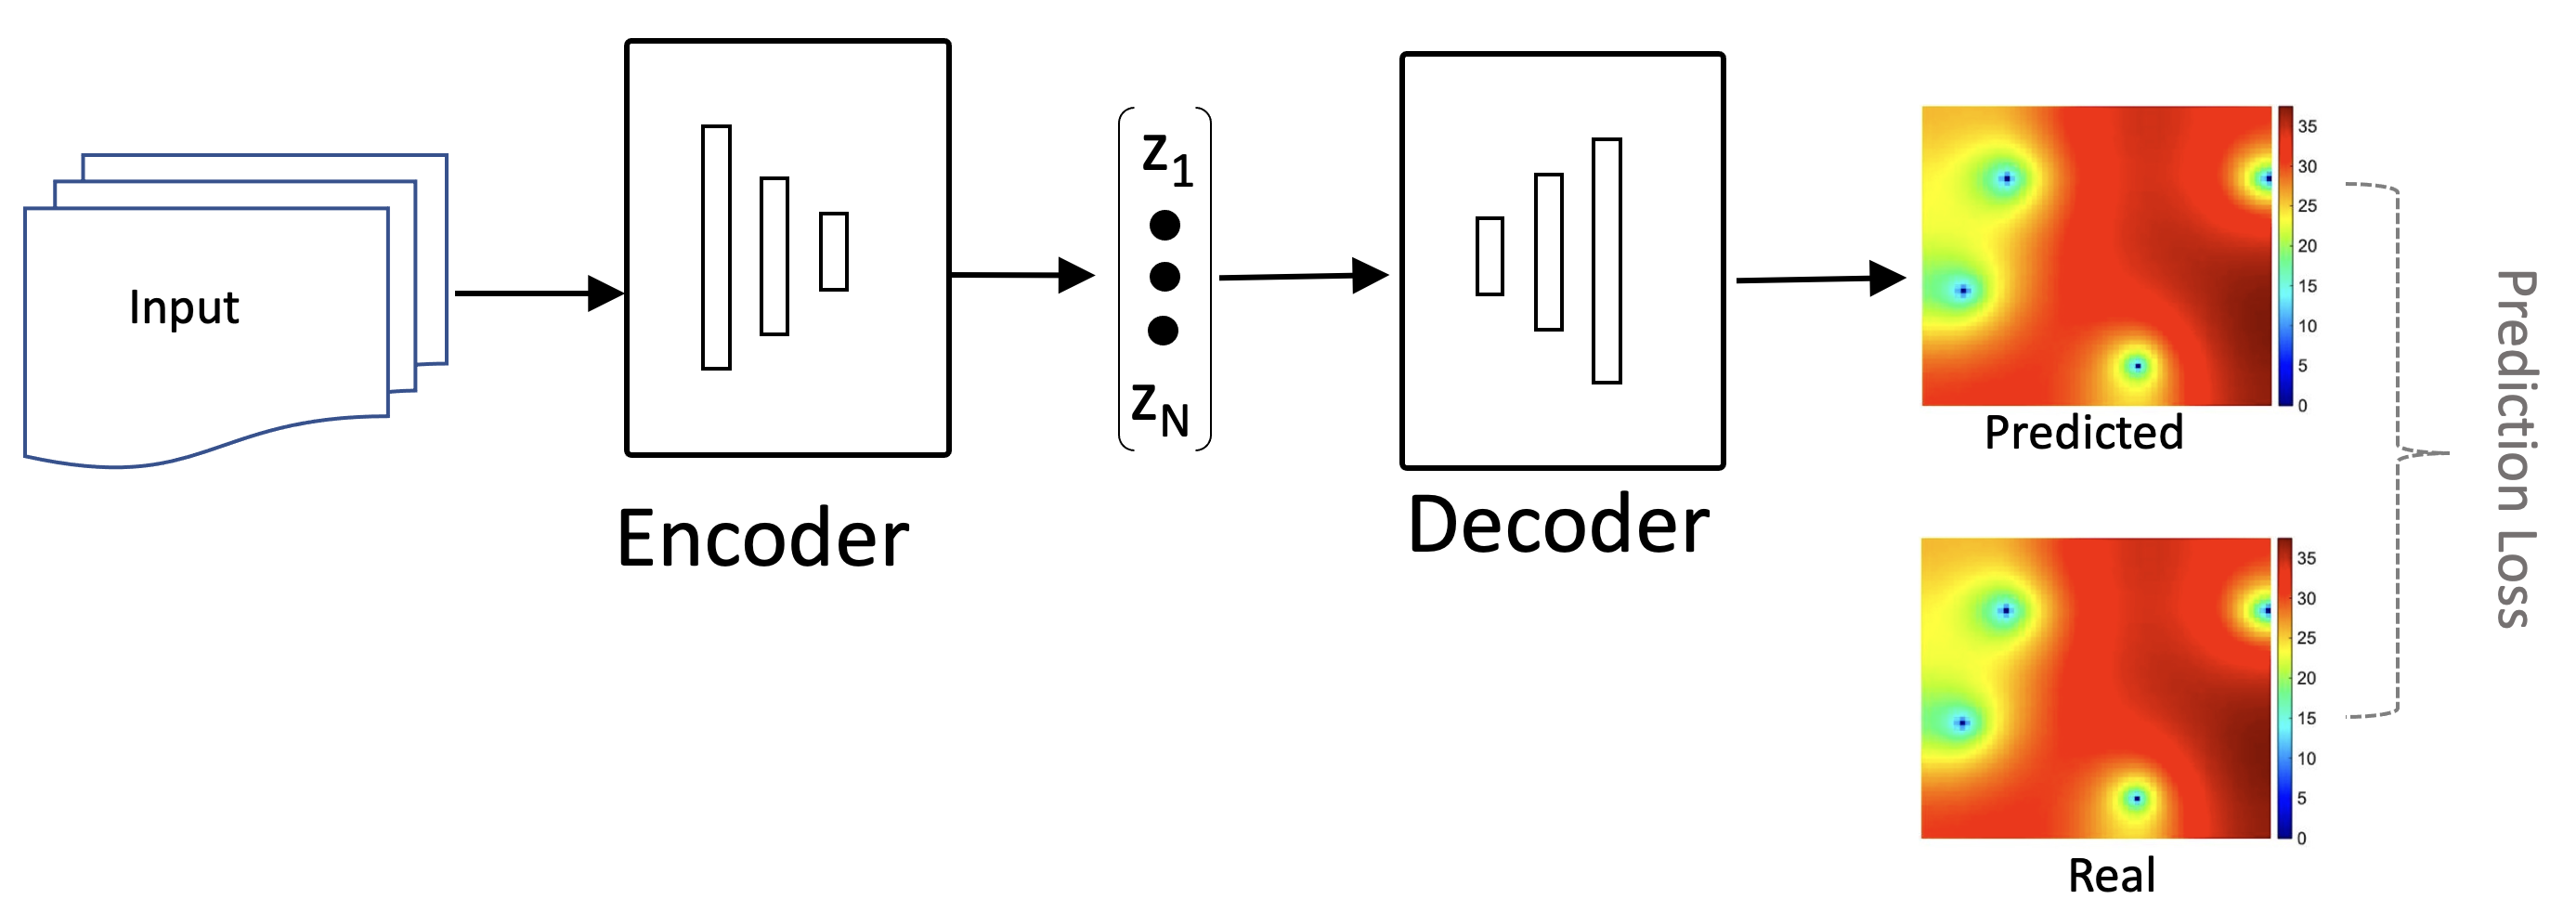
\includegraphics[width=0.9\columnwidth, height = 3cm]{./figs/ae_brief.eps}
		\label{fig:ae}}
	\subfigure[]{
		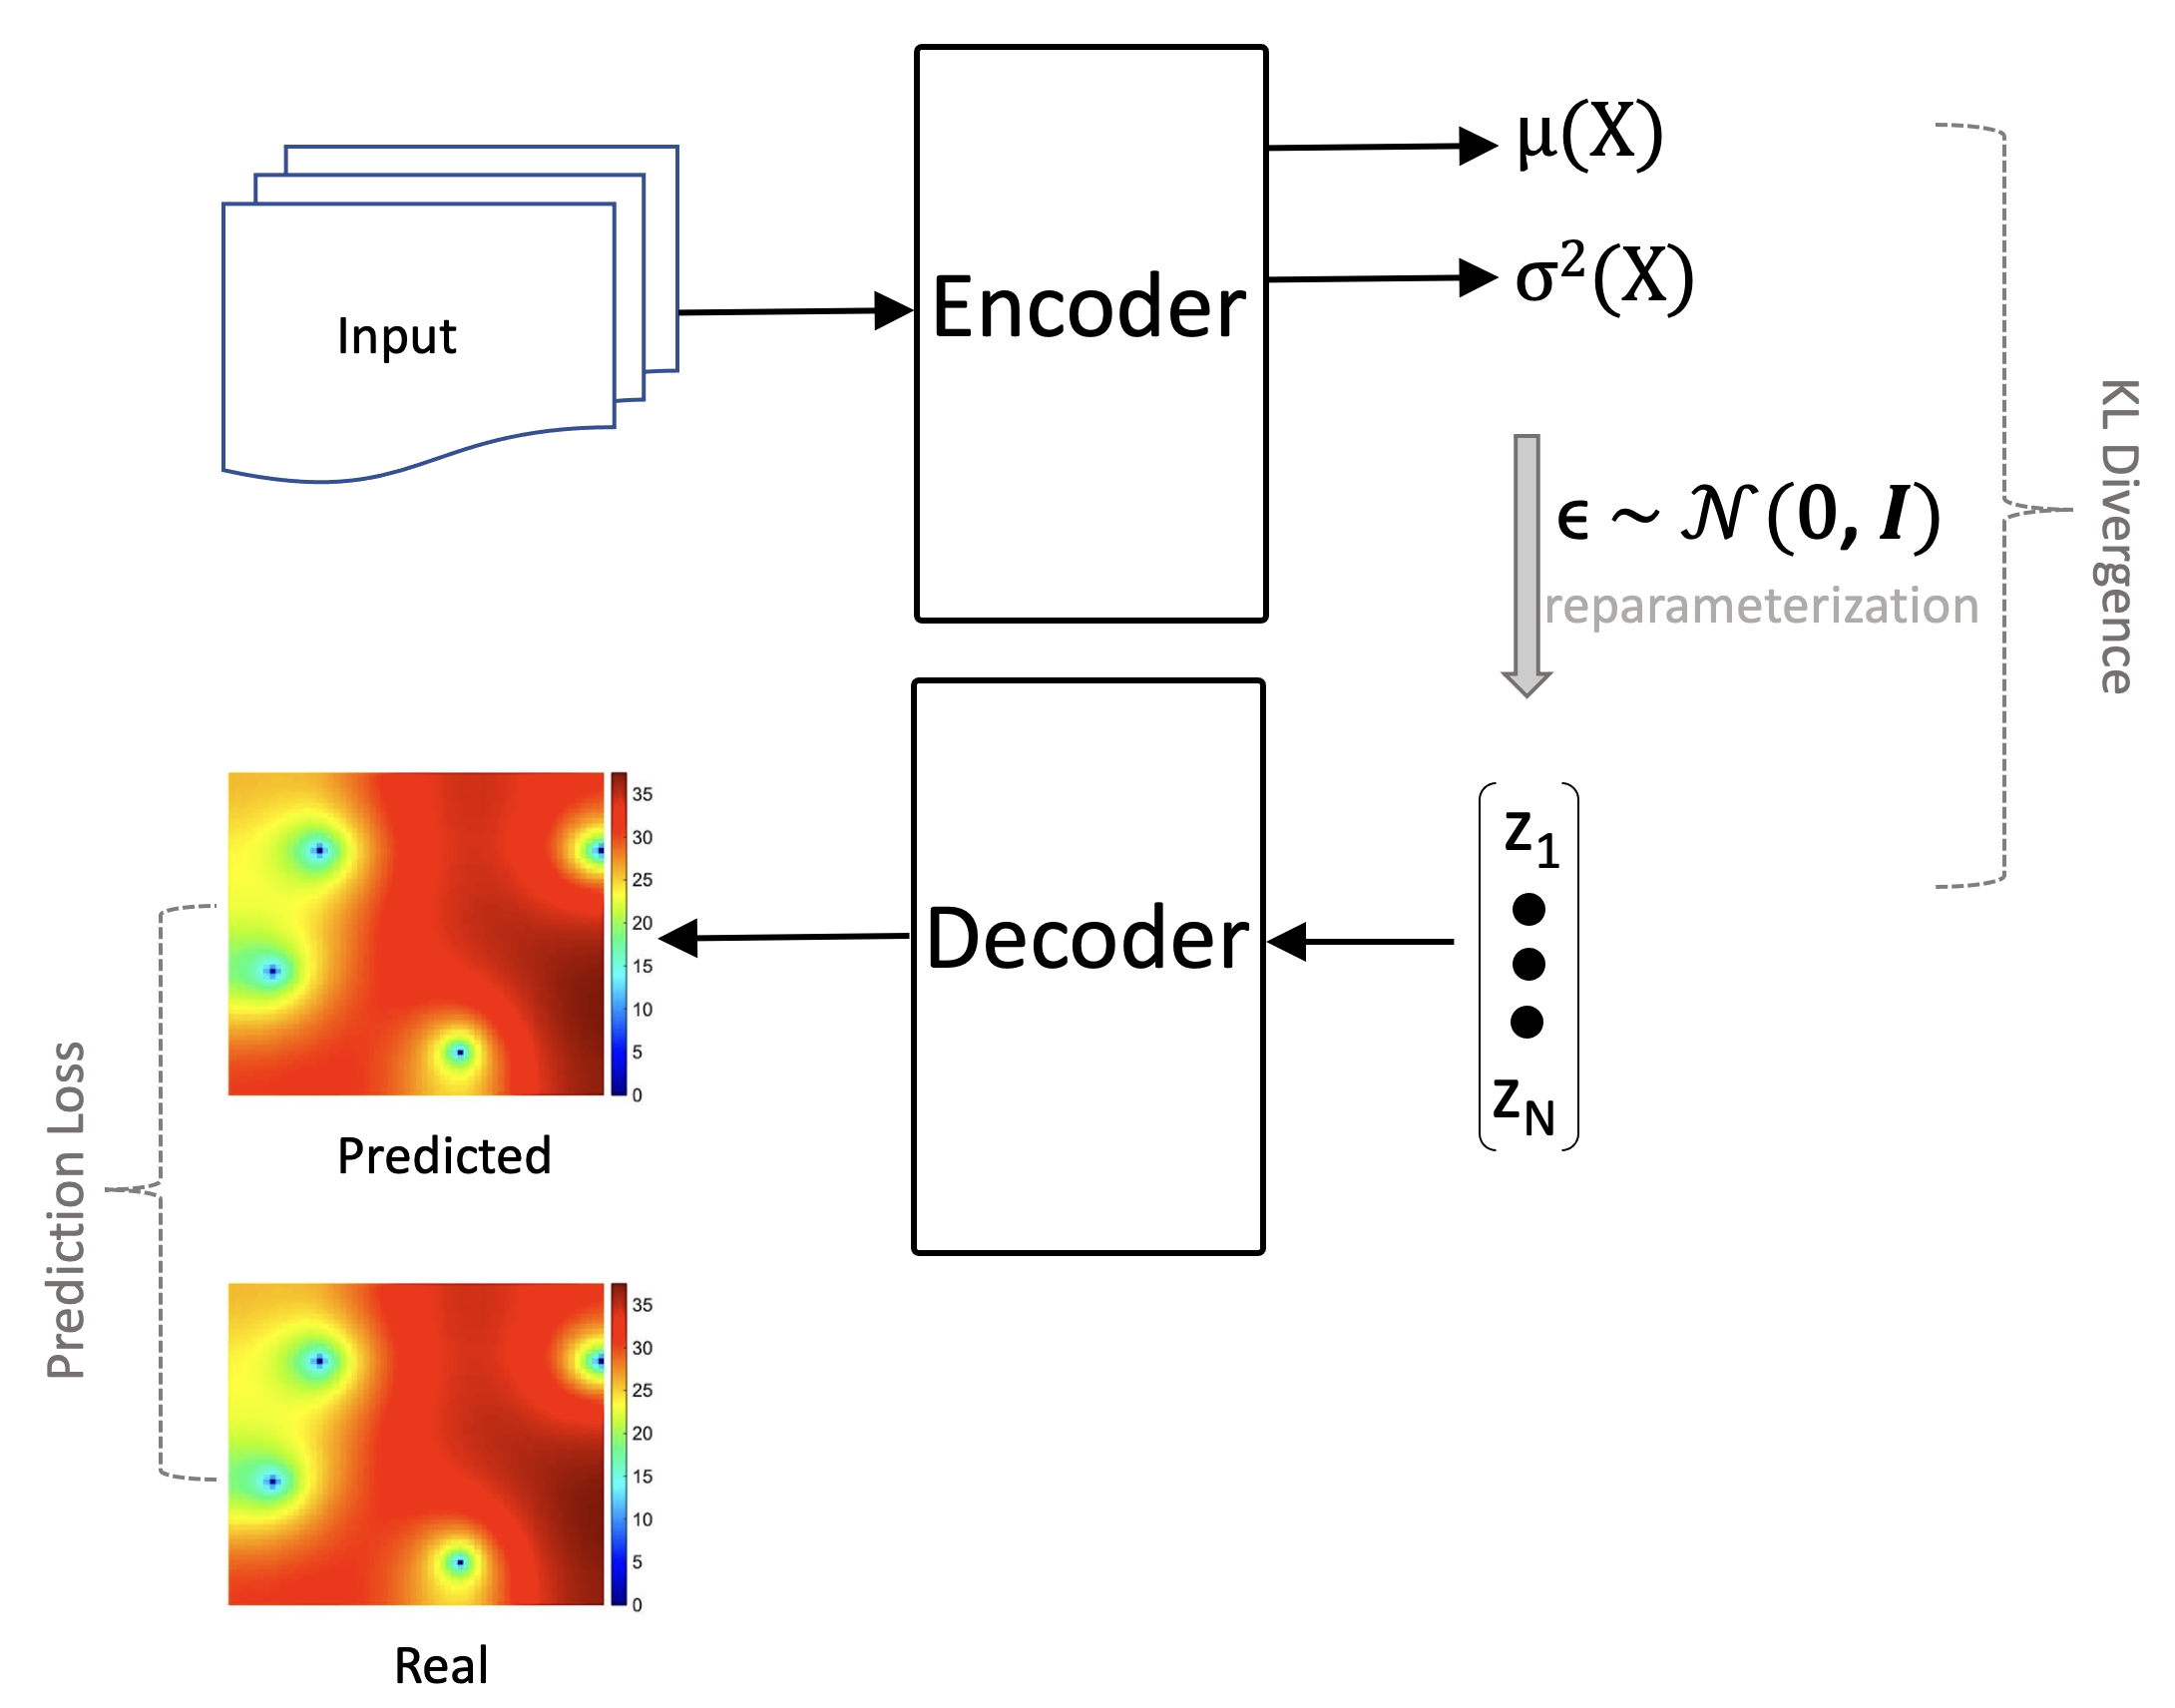
\includegraphics[width=0.8\columnwidth]{./figs/vae_brief.eps}
		\label{fig:vae}}
	\caption{(a) Architecture of an auto encoder (b)Architecture of a variational auto encoder }
	\label{fig:compare_ae_vae}
\end{figure}


\subsubsection{GridVAE Framework}
\label{subsubsec:vae}



\begin{figure*}[h!]
	\centering
	\includegraphics[width=1.8\columnwidth]{./figs/vae_detail.eps}
	\caption{The architecture of the proposed GridVAE for EM-aware IR drop prediction} 
	\label{fig:VAE_architecture}
\end{figure*}

The proposed GridVAE  is shown in Fig.~\ref{fig:VAE_architecture}. Take an example power grid design with 60 rows and 60 columns, the GridVAE model input consists of four channels, which are the power grid topology splitted into vertical conductance $\mathbb{R} ^{60\times 60\times 1}$ and horizontal conductance $\mathbb{R} ^{60\times 60\times 1}$,  the current source map $\mathbb{R} ^{60\times 60\times 1}$ drawn to other circuit layers, and a target lifetime $\textit{t}$ expanded into $\mathbb{R} ^{64\times 64\times 1}$ by channel-wise duplication. Since size 60 x 60 is close to 64 x 64, we padded 2 zero entries on each side of the input so that the model input size becomes 64 x 64 x 4.  In this example, the encoder consists of four convolutional layers followed by two fully-connected layers. if the power grid exceeds the size of 64 x 64 but is smaller than 128 x 128, we pad the input into the standard size of 128 x 128 and add one more convolutional layer in both the encoder and the decoder network.  Similarly, if the input dimension is larger than 128 but smaller than 256, we further pad the input to size 256 x 256 and add another one more convolutional layer. Thus the GridVAE model is actually quite scalable for larger power grid.

The input $\textit{\textbf{x}}$ is encoded to a 20-dimensional multivariate Gaussian distribution in the latent space. We denote the mean of $Q(Z|X)$ as  $\mu_{x}$   and the standard deviation as   $\sigma_{x}$ .
We use the reparameterization trick to ensure the model back propagation with gradient descent while sampling the latent variable, as shown in \eqref{eq:z_compute}, which first samples from $\epsilon \sim \mathcal{N}(\textbf{0}, \textbf{I} )$ and then computes the latent variable $\textit{\textbf{z}}$:
\begin{equation}
	\label{eq:z_compute}
	\textbf{z}  = \mu(\textit{X}) + \sigma \ast \epsilon(\textit{X})
\end{equation}

The decoder is designed to mirror the architecture of the encoder in a symmetric manner, except the output layer has only one channel. 
The output is $\mathbb{R} ^{64\times 64\times 1}$ EM-aware IR drop at target aging year.

\subsubsection{Training and Data Preparation}
The total loss function consists two parts. The first part is the \textit{reconstruction loss}, also called \textit{prediction loss} when the input and output are expected to differ. The \textit{prediction loss} measures the difference between the decoded result $\hat{y} = P(\hat{y}|z)$ and real data $y$, encouraging the decoded output data to be similar to the label. As our data is continuous, we allocate the mean squared error (MSE) for the \textit{prediction loss evaluation} in  \eqref{eq:vae_MSE_loss}, where N is the total number of output pixels.
\begin{equation}
	\label{eq:vae_MSE_loss}
	\textit{MSE}(y, \hat{y}) = \frac{1}{N} \sum_{1}^{N} ( y - \hat{y})^{2}
\end{equation}
The second part is the \textit{Kullback-Leibler (KL) divergence} between the encoder's latent variable distribution $Q(z|x)$ output and a chosen prior distribution, usually a standard multivariate Gaussian distribution $\mathcal{N}(\textbf{0}, \textbf{I})$. The \textit{KL divergence} measures how one probability distribution differs from a second, which acts as a regularization term to force the encoded latent variable distribution from the given training dataset to be close to a standard normal distribution, and encourage the network to use the latent space efficiently. 
The \textit{KL divergence} in VAE can be written as:

\begin{equation}
	\label{eq:vae_KLD_loss}
	D_{KL}( \mathcal{N}(\mu_{x}, \sigma_{x}^{2}) ~ || ~ \mathcal{N}(\textbf{0}, \textbf{I} ) )  = \dfrac{1}{2} (-\log\sigma^{2} + \mu^{2} + \sigma^{2} - 1)
\end{equation}

Hence the training target is to minimize the total loss:
\begin{equation}
	\label{eq:var_total_loss}
	\min  \{ \textit{MSE} (y, \hat{y})  ~ + ~ \lambda \cdot D_{KL}( \mathcal{N}(\mu_{x}, \sigma_{x}^{2}) ~ || ~ \mathcal{N}(\textbf{0}, \textbf{I} ) )  \}
\end{equation}
where $\lambda$ is the hyper parameter that adjusted similar to~\cite{Fu:arxiv'19} to prevent KL vanishing.

We measure the prediction accuracy in RMSE~\eqref{eq:RMSE}, the unit is mV
\begin{equation}
	\label{eq:RMSE}
	\textit{RMSE} =\sqrt{ \frac{1}{N} \sum_{1}^{N} ( y - \hat{y})^{2} }
\end{equation}






The data preprocessing before the model training is as follows:
First, the circuit layouts are automatically created by Synopsys IC compiler from a synthesized gate-level netlist and a standard cell library. 
Then IC Compiler output power grid information is sent to the power grid file parser, which reorganizes the information, including structure, wire layer, wire length, wire resistance values, node location, voltage, current source, etc.
Next, the $\it{EMspice}$ provides the EM-aware electrical information from the result above.
Eventually, we parse these EM-aware electrical features and the topological information for the circuit layout and send it to our VAE-based model for training and testing.  The inputs conductance and current are normalized

\begin{table}[!htbp]
	\begin{center}
		\caption{Power Grid Designs Detail}
		\label{table:pg_detail}
		%\vspace{-0.1in}
		\center
		\resizebox{0.48\textwidth}{!}{
		\begin{tabular}{ c | c | c | c | c}
			\hline 
			circuit &{\# nodes}&{\# Trees}&{\# voltage sources} &{$V_{DD}$ (V)}  \\ \hline 
			\hline 
			Design1 &1024 &64   &2 &1.05  \\ \hline
			Design2 &4096 &128  &4 &1.05 \\ \hline
			Design3 &16384 &256 &4 &1.05  \\ \hline
			Design4 &65536 &512 &9 &1.05  \\ \hline
		\end{tabular}
		}
	\end{center}
	\vspace{-0.1in}
\end{table}




\subsection{Fast power grid EM-aware IR drop fixing framework }
\label{subsec:formulation}

The proposed GridVAE-accelerated PDN IR drop fixing strategy's workflow is shown in Fig.~\ref{fig:flow}. 

%\begin{figure*}[h!]
%	\centering
%	\captionsetup{justification=centering, margin=3cm}
%	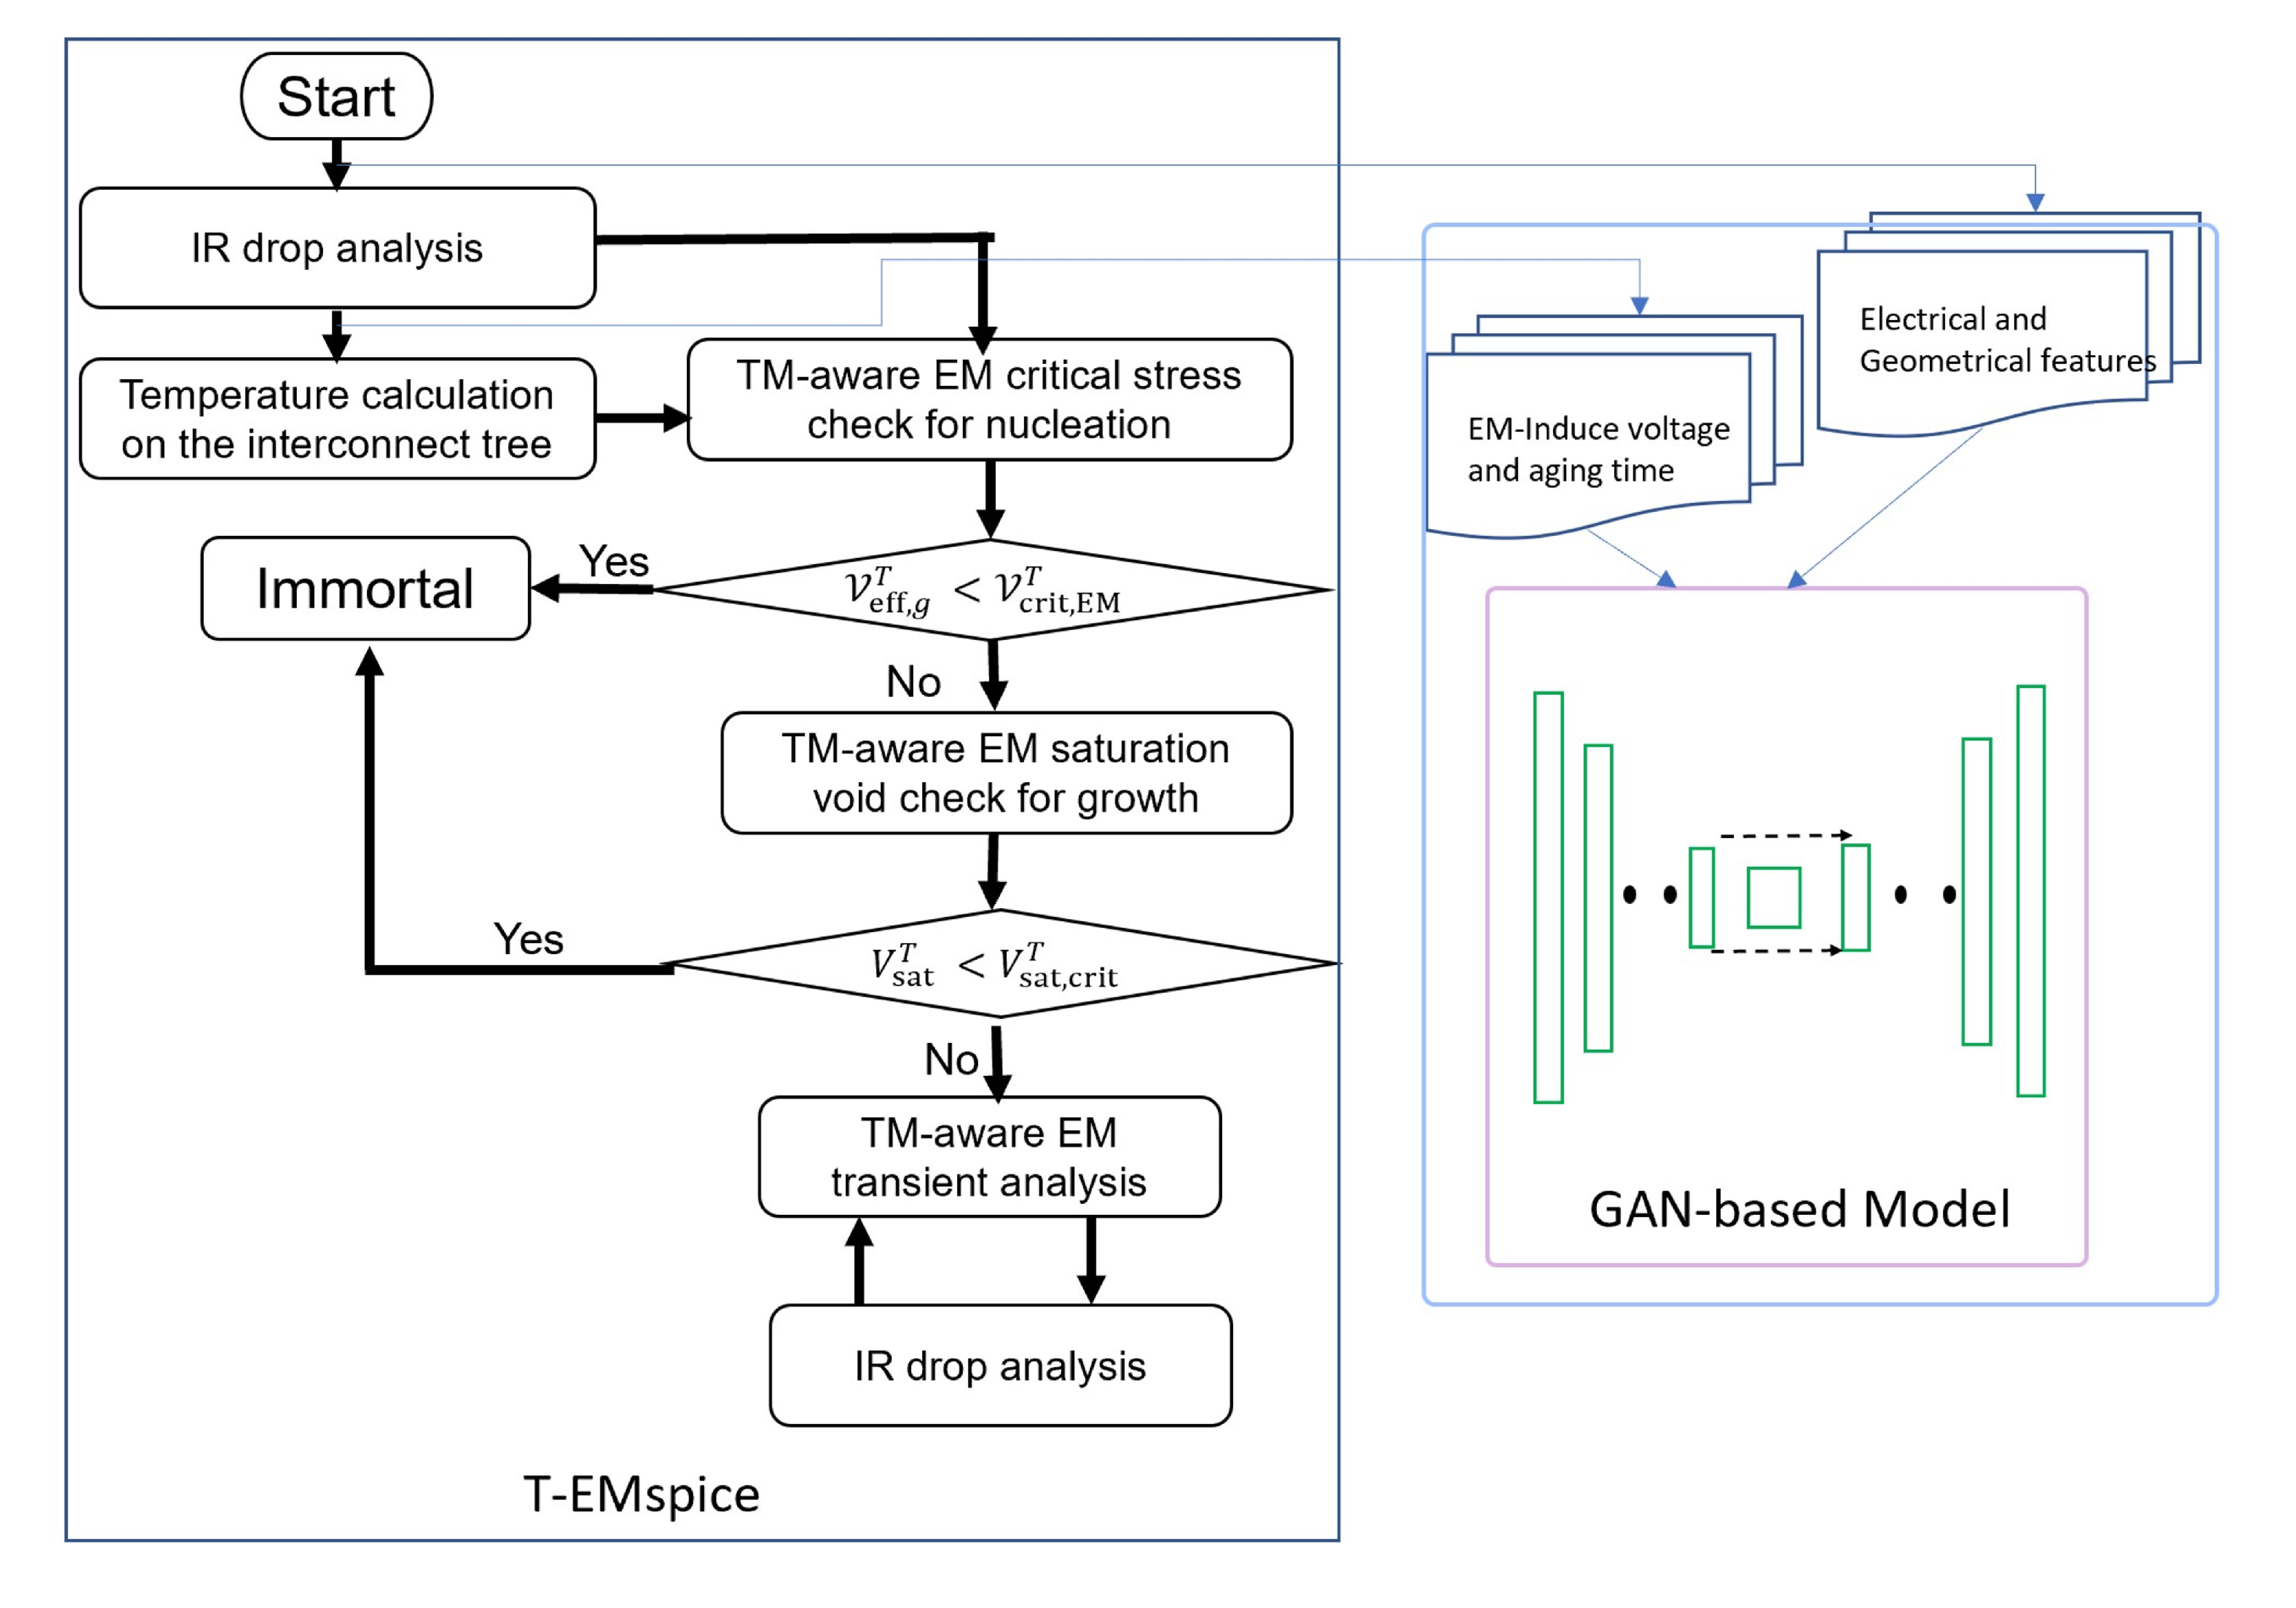
\includegraphics[width=1.2\columnwidth]{./figs/flow.eps}
%	\caption{The proposed framework of VAE-accelerated power gird fixing method.}
%	\label{fig:flow}
%\end{figure*}

\begin{figure}[h!]
	\centering
	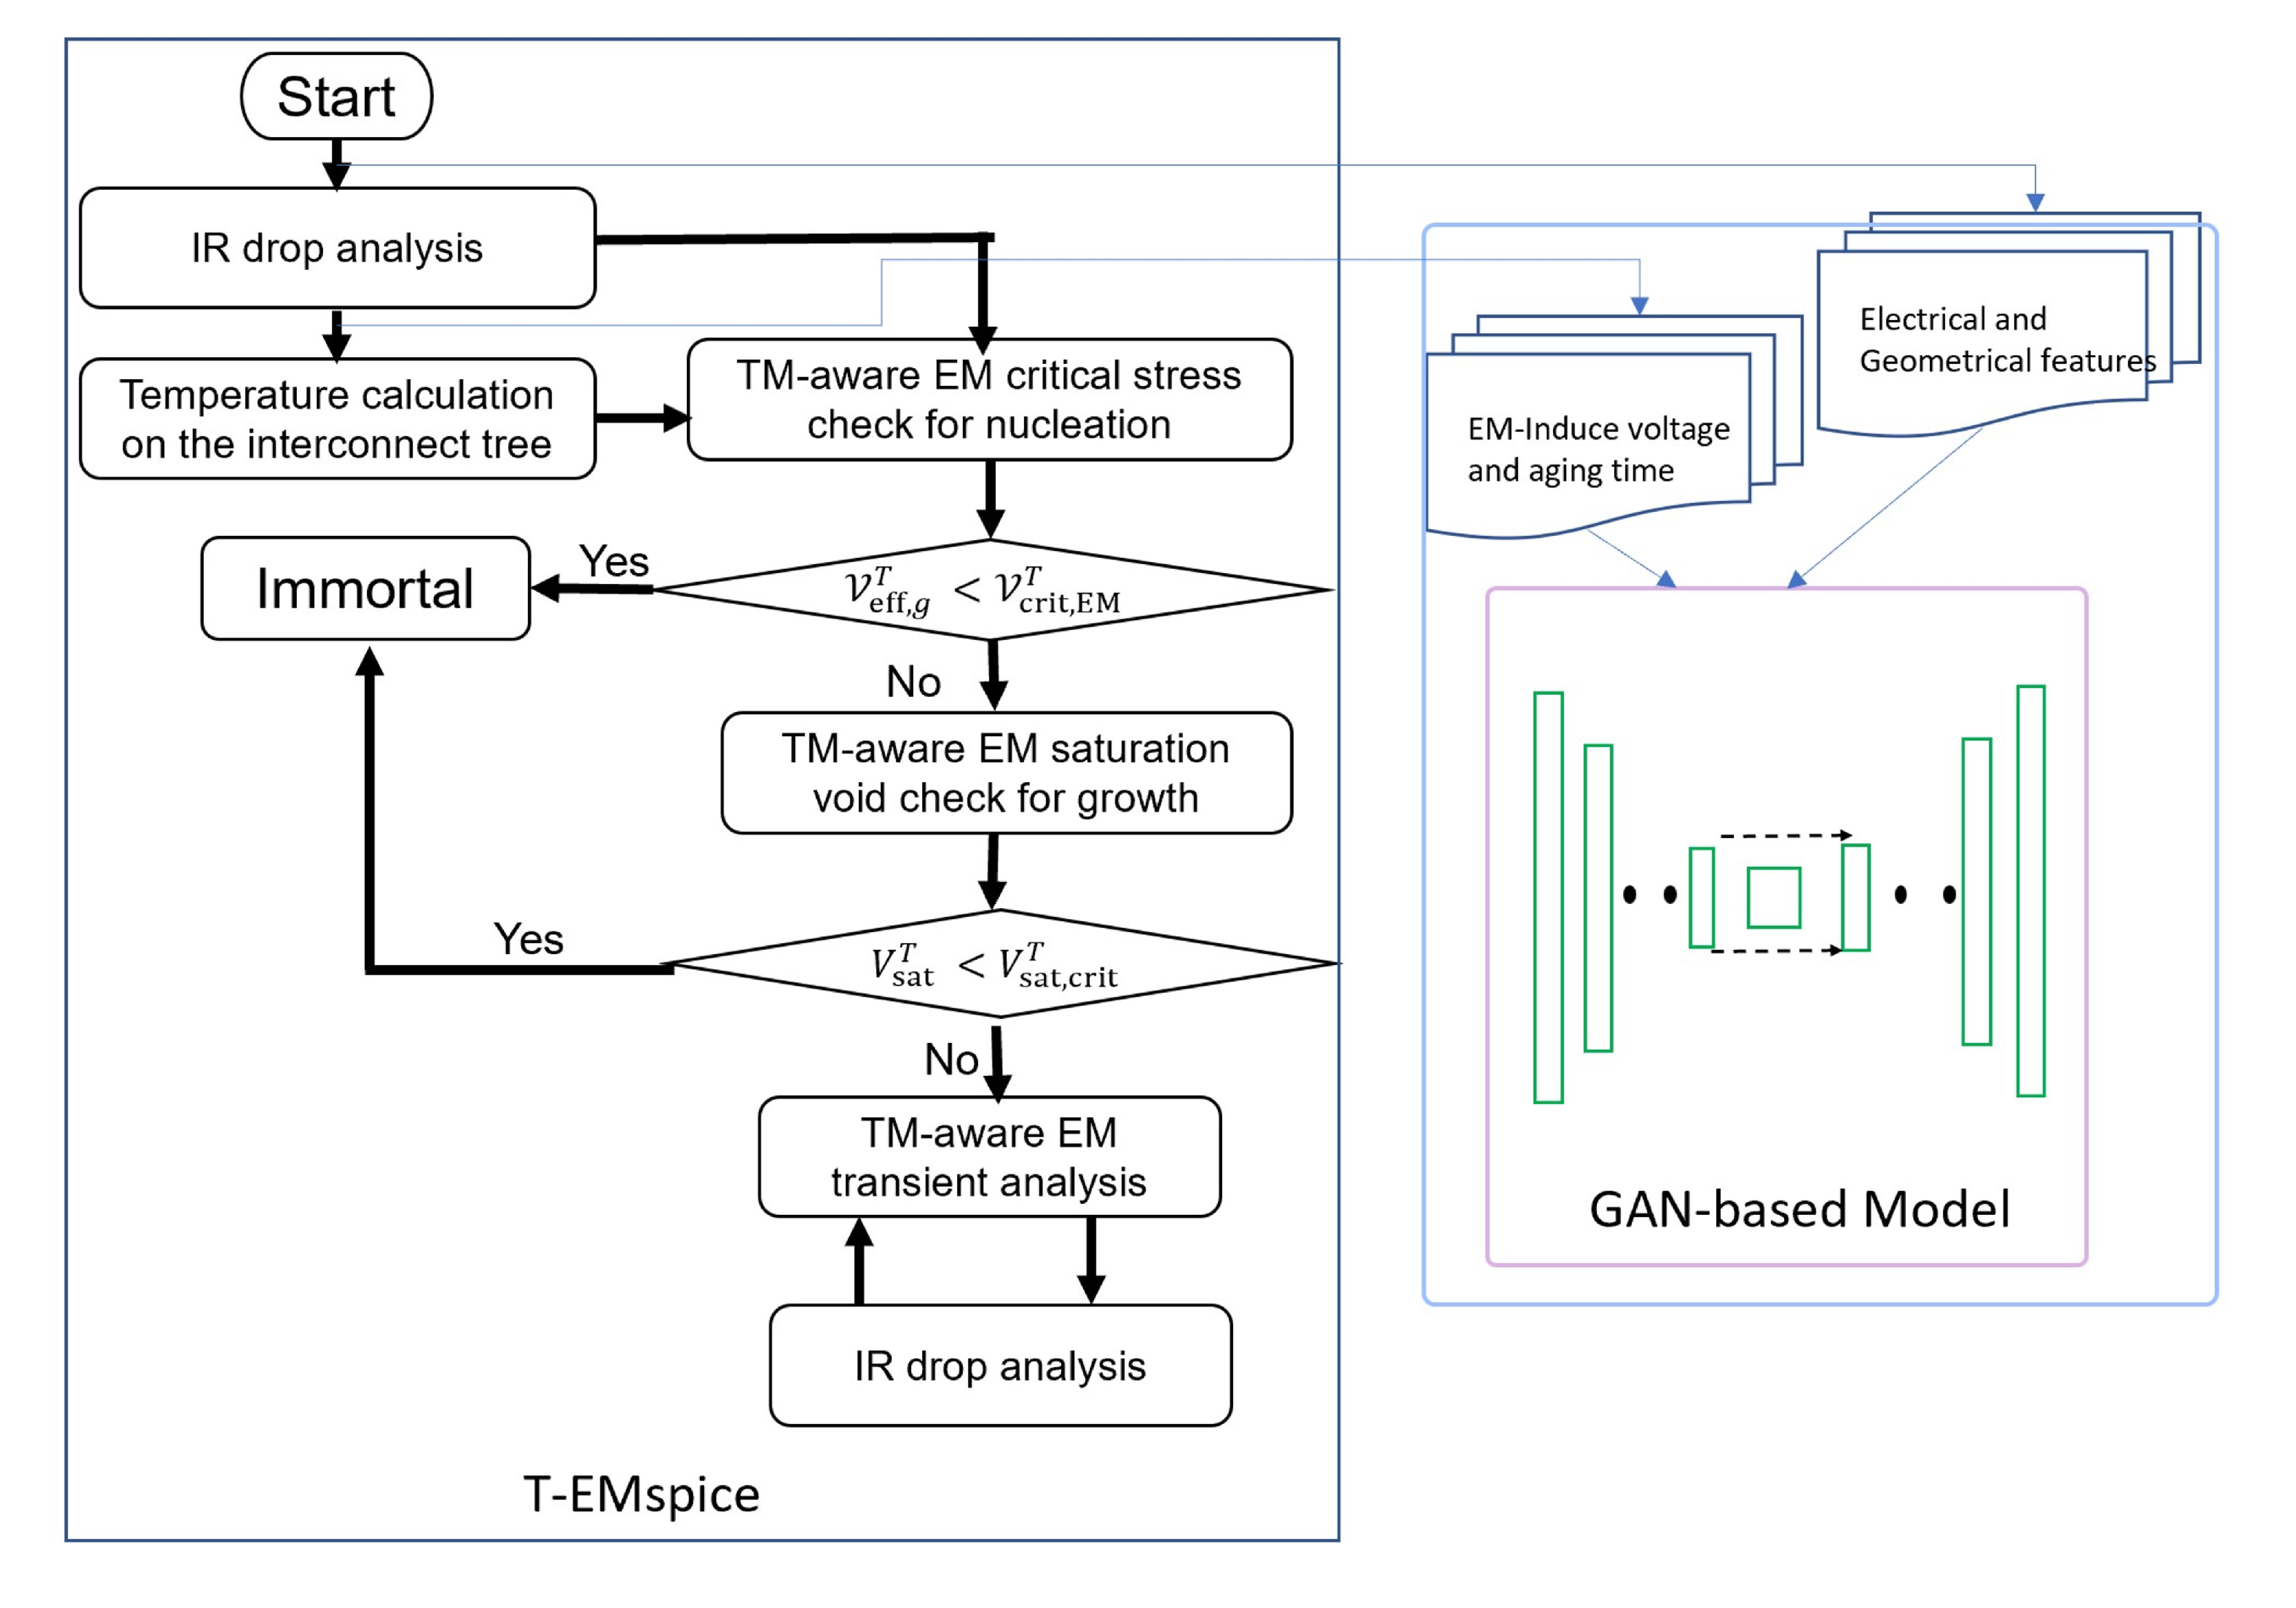
\includegraphics[width=0.98\columnwidth]{./figs/flow.eps}
	\caption{Framework of power gird IR drop fixing method accelerated by the GridVAE.}
	\label{fig:flow}
\end{figure}

\subsubsection{Problem formulation}
\label{subsubsec:formulation}
The proposed method intends to solve the following problem: 
Given the power grid information at T=0, the GridVAE has predicted the EM-aware IR drop at the target aging lifetime T = \textit{t} and revealed that the power grid has EM-induced IR drop violations demand fixing. IR drop violation means the power grid  has nodes voltage drop \textit{\textbf{v}} above the threshold $V_{th}$.
We wish to alleviate the above mentioned EM-aware IR drop failure by resizing the power grid interconnection trees' width with a minimum metal area increase.

The problem can be formulated as:
\begin{align}
	\label{eq:prob_formulation}
	&\mbox{Minimize}  & a^{t}s \qquad   \notag  \\
	&s.t.     & v(t,s)\leq V_{th} \\
	& \quad   &s \in S   \triangleq \{ s \in R^{nt}: 1 \leq s \leq s_{up} \}        \notag
\end{align}

In \eqref{eq:prob_formulation}, $a=[a_{1},a_{2},\ldots,a_{nt}] = [w_{1}l_{1},w_{2}l_{2},\ldots,w_{nt}l_{nt}]$ refers to the metal areas of the power grid with $n_{t}$ trees, $w_{i}$ and $l_{i}$ are the $i_{th}$ tree's width and length separately.
As for the constraint, $s=[s_{1},s_{2},\ldots,s_{nt}]$  is the resizing factor for the power grid trees. $S$ is the feasible region, where $s_{up}$ is the upper bound for $s$. Similar to~\cite{Sukharev:2019pg}, we assume the original power grid trees are already set to their minimum width. Hence we only increase the treewidth and $s \geq 1 $.
The feasible region reflects both the basic design rules and case-by-case user requirements, such as the criteria of minimum interconnect treewidth, the minimum spacing to prevent the interconnect trees overlap, and the maximum metal area usage, etc. 
The node IR drop $v(t,s)$ is the voltage difference between the power grid interconnect node and the power supply, it is a nonlinear function to $s$ at aging time $t$. The maximum allowable voltage drop threshold $V_{th}$ is given by the user. We assumed it to be five percent of the power supply voltage.


\subsubsection{Programming-based optimization}
\label{subsubsec:slp_framework}

As we mentioned in ~\ref{subsubsec:formulation}, the EM-aware PG node voltage drop $v(t,s)$ is a nonlinear function to $s$ at aging time $t$. Hence \eqref{eq:prob_formulation} is a nonlinear optimization problem. 
We solve it by a stepping strategy, in which we linearize the voltage drop at the current latest solution point by Taylor's expansion \eqref{eq:v_taylor_expand} and solve it with linear programming (LP) solver. We repeat this operation until the power grid has no EM-aware IR drop violation.

\begin{equation}
	\label{eq:v_taylor_expand}
	v(t, s^{(i+1)}) \triangleq v(t,s^{(i)}) + \dfrac{\partial v(t, s^{(i)})}{\partial s} \cdot \delta s
\end{equation}
where $s^{(i)}$ denotes the current power grid resizing vector and $s^{(i+1)}$ is defined as 
\begin{equation}
	\label{eq:s}
	s^{(i+1)} = s^{(i)} + \delta s 
\end{equation}

$ \dfrac{\partial v(t, s)}{\partial s}$ is the $n\times n_{t}$ \textit{Jacobian} matrix of $v(t,s)$ with respect to $s$, describes how the node voltage drops at target time $T=t$ respond to the corresponding treewidth rescaling.

\begin{equation}
	\label{eq:J_matrix}
	\dfrac{\partial v(t, s)}{\partial s}=
	\mathbf {J}_{n\times n_{t}}(s,t) =
	\begin{bmatrix}
		\frac{\partial v(1,t)}{\partial s_{1}}&\frac{\partial v(1,t)}{\partial s_{2}}&\ldots&\frac{\partial v(1,t)}{\partial s_{n_{t}}}\\
		\frac{\partial v(2,t)}{\partial s_{1}}&\frac{\partial v(2,t)}{\partial s_{2}}&\ldots&\frac{\partial v(2,t)}{\partial s_{n_{t}}}\\
		\vdots&\vdots&\ddots&\vdots\\
		\frac{\partial v(n,t)}{\partial s_{1}}&\frac{\partial v(n,t)}{\partial s_{2}}&\ldots&\frac{\partial v(n,t)}{\partial s_{n_{t}}}
	\end{bmatrix}
\end{equation}



\subsubsection{Fast gradient computation via auto differentiation}
PyTorch auto differentiation can provide the gradient of output node voltages to the input wire segment conductances, which is $ \dfrac{\partial v(t, s)}{\partial g}$. Then we can quickly get \eqref{eq:J_matrix} by chain rule, as each power grid tree $g_{i}$ has its resizing factor $s_{i}$ and will not be infected by other resizing factors:
\begin{equation}
	\label{eq:chain_rule}
	\begin{aligned}
	\begin{split}
	\frac{\partial v}{\partial s} & =\frac{\partial v}{\partial g} \frac{\partial g}{\partial s}, \\ 
	\frac{\partial g_{i}}{\partial s_{k}} & = 
    	\begin{cases}
        		0,      &\mbox{if i $\neq$ k} \\ 
        		g_{i},  &\mbox{if i = k} 
    	\end{cases}
	\end{split}
	\end{aligned}
\end{equation}

As a comparison to the sensitivity acquisition by matrix solving method~\cite{Sukharev:2019pg}, we briefly review its main steps.
For a power grid network represented by the node conductance matrix $ \textit{G(t,s)}$, it can be written in the following format~\eqref{eq:gv=i}:
\begin{equation}
	\label{eq:gv=i}
	G(t,s)\cdot v(t,s)= j(t)
\end{equation}
where $j(t)$  is $n\times 1$ vectors representing and node current vector for the power grid.

And the sensitivity is calculated as followed~\eqref{eq:dVs}: 
\begin{equation}
	\label{eq:dVs}
	\dfrac{\partial v(t,s)}{\partial s_{k}} = -G^{-1}\cdot \dfrac{\partial G(t,s)}{\partial s_{k}}  \cdot G^{-1}\cdot j(t)
\end{equation}

To solve the above equation and obtain $ \frac{\partial v(t,s)}{\partial s_{k}}$, one must first construct the sparse matrices G and $\frac{\partial G(t,s)}{\partial s_{k}}$ for all $k$, then perform matrix solving. 
Each column of the \textit{Jacobian} matrix \eqref{eq:J_matrix} has to be calculated through the process of \eqref{eq:dVs} for the corresponding power grid tree. Hence building such a \textit{Jacobian} matrix in the traditional method is computationally expensive.










